In order to find the most suitable algorithm for translating a live input stream of American SLA to any other suitable SLA (sharing the same alphabet) in a real-world application, the algorithm needs to excel in two main aspects: accuracy and inference time. A third factor that may come into question here is the training time, as computational cost may accumulate when further improving the model in the future.

\subsection{Result from the long list}
As mentioned in chapter \ref{chapter_models} the long list contained 27 pretrained models. Due the the limited availability of computational ressources, the models on the list as per table \ref{tab:keras_models} (including all variants) were trainined in an experimental setup, to determine which models are suitable for a full training. The goal was to use these pretrained models and only train the last layer to enable the detection of SLA in sources such as webcam feeds, videos or images.

The experimental setup was trained on a consumer pc, with a 3.8 Ghz 6-core CPU, a \textit{GeForce GTX 1060} GPU and 32GB of RAM. The results mainly focus on two aspects in order to decide which models may be suitable for the full training: training time and accuracy. As shown in Fig. \ref{fig:long_list_acc} some of the models already have a high accuracy with a minified training.

\begin{figure}[h]
    \centering
    \caption{Accuracy on long list training}
	\label{fig:long_list_acc}
    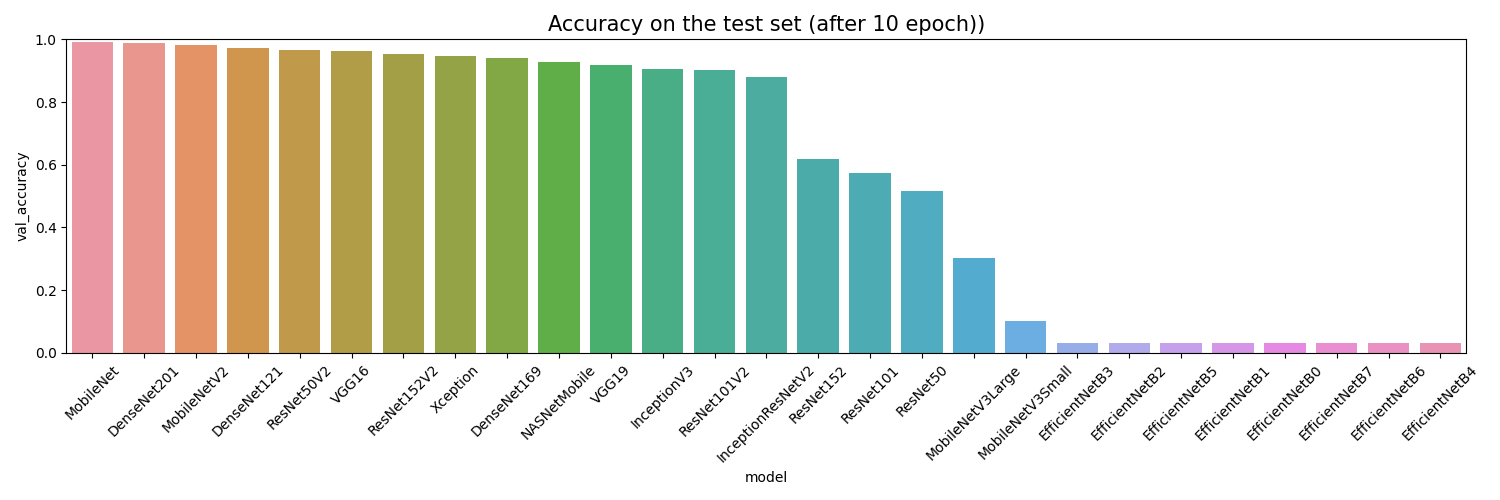
\includegraphics[width=\linewidth]{figures/long_val_accuracy.png}
\end{figure}

While models as \textit{DenseNet} seem to have good results with all variants, others like \textit{ResNet} have a high variety, accuracy ranges from ~55\% (\textit{ResNet50}) to ~98\% \textit{ResNet50V2}. The \textit{EfficientNet} with all its variants has an accuracy below 10\% and will not move forward.

\begin{figure}[h]
    \centering
    \caption{Training time on long list training}
	\label{fig:long_list_time}
    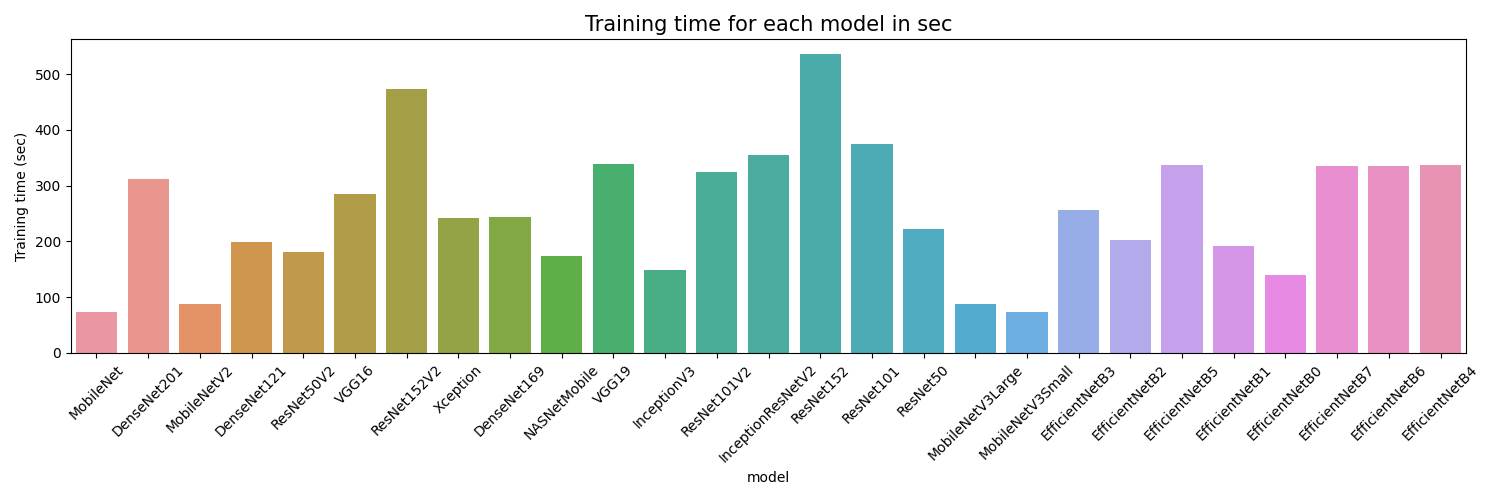
\includegraphics[width=\linewidth]{figures/long_training_time.png}
\end{figure}

Fig. \ref{fig:long_list_time} shows the time that was needed to train the models with the reduced dataset for 10 epochs without early stopping. To determine, whether a model should be used for the full training, we calculated the ratio of accuracy and training time and normalized the results between 0 and 1 with the formula

\begin{equation}
    z_i=\frac{x_i - min(x)}{max(x) - min(x)}
\end{equation}
having \begin{math} x_n = accuracy_n / time_n \end{math} and \begin{math}x \in \mathbb{N} = \{0,...\}\end{math}. Shown in Table \ref{tab:result:long} are the top 10 normalized ratios for the trained models of the long list. 

\begin{table}[th]
    \caption{Top 10 Long List Results}
    \label{tab:result:long}
    \centering
    \begin{tabular}{@{}llll@{}}
    \toprule
    Model & \begin{math}accuracy\end{math} & \begin{math}time\end{math} & \begin{math}z\end{math} \\ \midrule
    1    & 0.99 & 121s                                                      & 0.69                                                  \\
    3    & 0.98 & 165s                                                      & 0.51                                                  \\
         &      &                                                          &                                                       \\
         &      &                                                          &                                                       \\
         &      &                                                          &                                                       \\
         &      &                                                          &                                                       \\
         &      &                                                          &                                                       \\
         &      &                                                          &                                                       \\ \bottomrule
    \end{tabular}
\end{table}

\subsection{Result from the short list}

\subsection{Result from the prediction and translation}
